\documentclass[t,table,usenames,dvipsnames]{beamer}

\usetheme{CambridgeUS}
\usecolortheme{beaver}
\setbeamertemplate{navigation symbols}{}

\usepackage[utf8]{inputenc}
\usepackage[croatian]{babel}

\usepackage{datetime}
\renewcommand{\dateseparator}{.}
\newcommand{\todayiso}{\twodigit\day \dateseparator \twodigit\month \dateseparator \the \year}
\date{\todayiso}
\newcommand{\shell}[1]{\texttt{#1}}


\usepackage{listings}
\usepackage{graphicx}
\usepackage{subcaption}
\usepackage{multirow}
\usepackage{color}
\definecolor{LightGray}{gray}{0.9}
\captionsetup{compatibility=false}

\title[NKOSL]{Napredno korištenje operacijskog sustava Linux}
\author[Leonard Volarić Horvat, Borna Skukan]{Leonard Volarić Horvat, Borna Skukan\\{\small Nositelj: doc.dr.sc. Stjepan Groš}}
\subtitle{4. Sistemski logovi i nadziranje}
\institute[FER]{Sveučilište u Zagrebu\\Fakultet elektrotehnike i računarstva}

\begin{document}
{
    \setbeamertemplate{footline}{}
	\begin{frame}
		\maketitle
	\end{frame}
}

\begin{frame}
    \frametitle{Sadržaj}
    \tableofcontents
\end{frame}

\section{Logging}

\begin{frame}
    \topskip0pt
    \vspace*{\fill}
        \begin{center}
            \Huge{Logging}
        \end{center}
    \vspace*{\fill}
\end{frame}


\begin{frame}
    \frametitle{Logovi}
    \begin{itemize}
        \item Dnevničke datoteke 
        \begin{itemize}
            \item tekstualne
            \item binarne (systemd dnevnički sustav: journald; journalctl)
        \end{itemize}
        \item Zapisuju radnje vezane za praćeni proces
        \item Primjena: dijagnoza kvarova, praćenje stanja sustava, kronologija događaja, sigurnosni zapisi...
    \end{itemize}
\end{frame}



\begin{frame}
    \frametitle{/var/log direktorij}
    \begin{itemize}
        \item Direktorij s glavninom log datoteka na sustavu
        \item Primjeri:
        \begin{itemize}
            \item boot.log - boot poruke
            \item auth.log - poruke o autentikacijama korisnika
            \item dpkg.log - poruke vezane uz dpkg (npr. \shell{apt install paket})
        \end{itemize}
        \item S dolaskom systemd-a dio logova prelazi iz /var/log u journalctl
    \end{itemize}
\end{frame}


\begin{frame}
    \frametitle{Syslog}
    \begin{itemize}
        \item Sustav koji hvata sve poruke u Linux sustavu
        \item Vrlo složena arhitektura, ugrađena u sve distribucije
        \item rsyslog (Reliable Syslog) - moderna verzija sysloga
        \item Daemon proces, jednostavan za korištenje
        \item Konfiguracija u /etc/\textbf{[r]}syslog.conf
    \end{itemize}
    \begin{itemize}
        \item Danas dijelom zasjenjen journald-om
        \item I dalje moguće paralelno koristiti oba
    \end{itemize}
\end{frame}

\begin{frame}
    \frametitle{/etc/syslog.conf}
    \begin{itemize}
        \item item.priority [; item.priority]   /path/to/file
    \end{itemize}

    \begin{columns}
        \begin{column}{0.5\textwidth}
           Vrsta: \\
            \begin{itemize}
                \item auth, authpriv (general and private auth)
                \item cron
                \item kern (kernel)
                \item mail
                \item news
                \item user (user process)
                \item uucp
                \item local\{0..\}
                \item ...x
            \end{itemize}
        \end{column}
        \begin{column}{0.5\textwidth}  %%<--- here
            Prioritet: \\
            \begin{itemize}
                \item emerg
                \item alert
                \item crit
                \item err
                \item warning
                \item notice
                \item info
                \item debug
                \item none
            \end{itemize}
        \end{column}
        \end{columns}

\end{frame}

\begin{frame}[fragile]
    \frametitle{/etc/syslog.conf}
    \begin{itemize}
        \item item.priority [; item.priority]   /path/to/file
    \end{itemize}
    \begin{verbatim}

    # All info, none mail nor privat auth
    *.info; mail.none; authpriv.none    /var/log/messages

    # Everybody gets emergency messages
    *.emerg                             *
    *.emerg                             @10.1.1.254
    
    # " = " will force ONLY specific priorty
    news.=crit                          /var/log/news/critical

    \end{verbatim}

\end{frame}

\begin{frame}[fragile]
    \frametitle{Logger utility - API to syslog}

    \begin{itemize}
        \item Korištenje iz drugih programa

        \item \shell{logger [options] [message]}
        \item Ispisuje poruku u /var/log/syslog

        \item \shell{Ožu 31 09:51:05 rincewind-N551JK rincewind[569]: This is the Central Scrutinizer}

    \end{itemize}

\end{frame}

\begin{frame}[fragile]
    \frametitle{Logrotate}
    \begin{itemize}
        \item Održavanje logova
        \item \shell{/etc/logrotate.conf} \shell{/etc/logrotate.d/}
    \end{itemize}

    \begin{verbatim}

    # rotate
    weekly
    # keep [weeks]
    rotate 4
    # create new after rotation
    create
    # compress
    compress
    # additional
    include /etc/logrotate.d

    \end{verbatim}

\end{frame}

\begin{frame}[fragile]
    \frametitle{Logrotate}
    \begin{itemize}
        \item Specifična datoteka
    \end{itemize}
    \begin{verbatim}
    # /etc/logrotate.d/nginx
    /var/log/nginx/*.log {
        daily
        missingok
        rotate 52
        compress
        delaycompress
        notifempty
        create 640 nginx adm
        sharedscripts
        postrotate
                [ -f /var/run/nginx.pid ] && 
                    kill -USR1 `cat /var/run/nginx.pid`
        endscript
    }

    \end{verbatim}

\end{frame}

\section{Monitoring}
\begin{frame}
    \topskip0pt
    \vspace*{\fill}
        \begin{center}
            \Huge{Monitoring}
        \end{center}
    \vspace*{\fill}
\end{frame}


\begin{frame}
	\frametitle{ps}
	
	\begin{itemize}
		\item "\textbf{p}rocess \textbf{s}tatus"
		\item Alat za prikaz trenutno aktivnih procesa
		\item Često koristen u kombinaciji s grep-om
	\end{itemize}
		 \shell{ps aux  \newline
				ps -ejH}		
	
		
	
\end{frame}

\begin{frame}
	\frametitle{top}
	
	\begin{itemize}
		\item \textit{Realtime} praćenje trenutnih procesa
		\item Mogućnost sortiranja i filtriranja
		\item Prikazuje i osnovne metrike o sustavu
		\item \shell{ htop } - intuitivniji i pregledniji
	\end{itemize}
\end{frame}

\begin{frame}
    \frametitle{htop}
    \begin{figure}
        \centering
        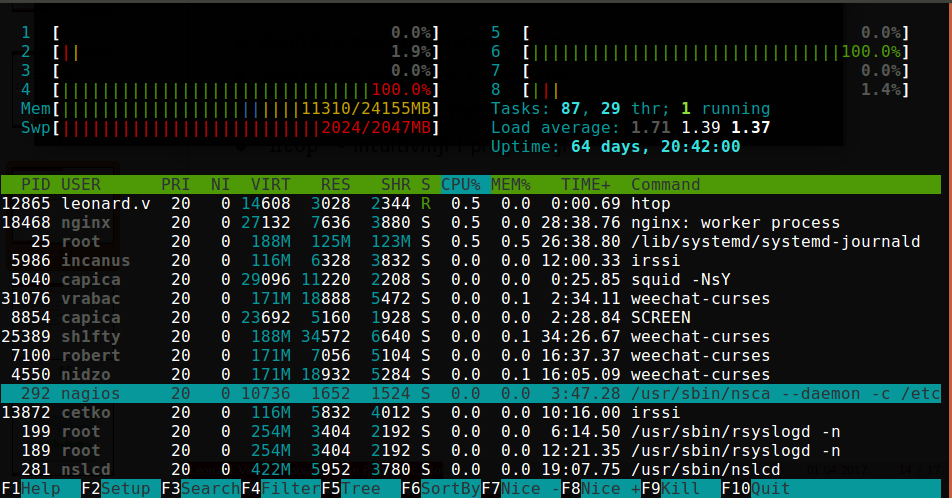
\includegraphics[width=1.0\linewidth]{htop-marvin}
        \caption{htop}
        \label{fig:htop-marvin}
    \end{figure}
\end{frame}

\begin{frame}
    \frametitle{/proc}
    \begin{itemize}
        \item Direktorij /proc - izvor većine podataka o procesima
        \begin{itemize}
            \item \shell{uptime - /proc/uptime}
            \item \shell{loadavg - /proc/loadavg}
            \item \shell{proces s traženim PID-om - /proc/\textless PID\textgreater}
        \end{itemize}
        \item /proc koristi \shell{procfs} pseudo-filesystem
        \item Dinamička struktura - stvara i briše pripadajuće datoteke zajedno s procesima
    \end{itemize}
\end{frame}

\begin{frame}
    \frametitle{Još neki alati}
    \begin{itemize}
        \item strace 
        \begin{itemize}
            \item Praćenje sistemskih poziva i signala
            \item Može se doznati odakle neki proces dobiva informacije
            \item \shell{strace uptime 2\textgreater\&1 | grep open} \\
        \end{itemize}
        \item iotop - top za IO operacije
        \item iostat - statistika o IO uređajima
        \item atop - top za "sve"
        \item netstat, ss - mrežni dijagnostički alati
    \end{itemize}
\end{frame}

\begin{frame}
	\frametitle{Nadzor procesa i sustava}
	
	\begin{itemize}
		\item Zabbix - agent + server + vizualizacija
        \item Ossec - Nadzor logova + mail
        \item Sentry - Ossec + akumulacija
		\item Sentry - agent + server + plugins
		\item Kibana - vizualizacijski alat
        \item Grafana, Prometheus
	\end{itemize}
	
\end{frame}

\begin{frame}
	\frametitle{Zabbix}
	\begin{figure}
		\centering
		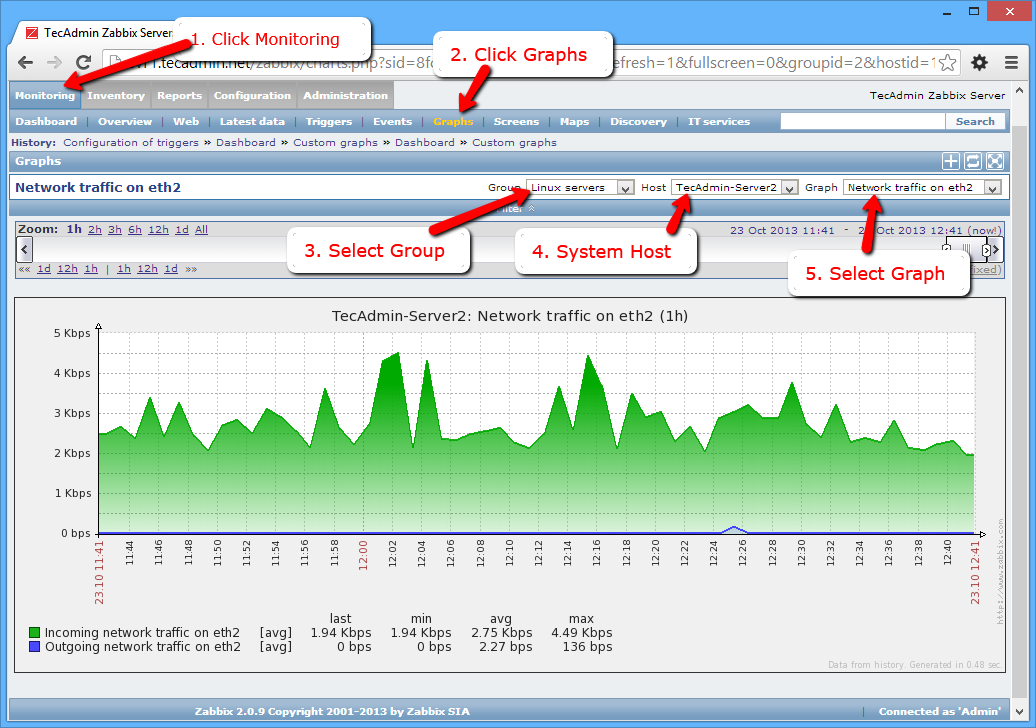
\includegraphics[width=0.7\linewidth]{graph-network}
		\caption{Zabbix}
		\label{fig:graph-network}
	\end{figure}
	
\end{frame}


\begin{frame}
	\frametitle{Literatura}
	\url{https://peteris.rocks/blog/htop/}
	\vfill
	\url{http://www.linuxcommand.org/man_pages/logrotate8.html}\\
	\url{http://man7.org/linux/man-pages/man3/syslog.3.html}\\
	\vfill
	\url{http://www.zabbix.com}\\
	\vfill
	\url{https://www.elastic.co/products/kibana}\\
    \vfill
    \url{https://www.cyberciti.biz/tips/top-linux-monitoring-tools.html}
\end{frame}

\end{document}
